\textbf{COLUNI 2020 -- Questão 34}\par\medskip Observe e analise o quadro abaixo sobre fluxos migratórios.

% COLUNI-AUTO-FIGURES-BEGIN
\begin{figure}[htbp]
\centering
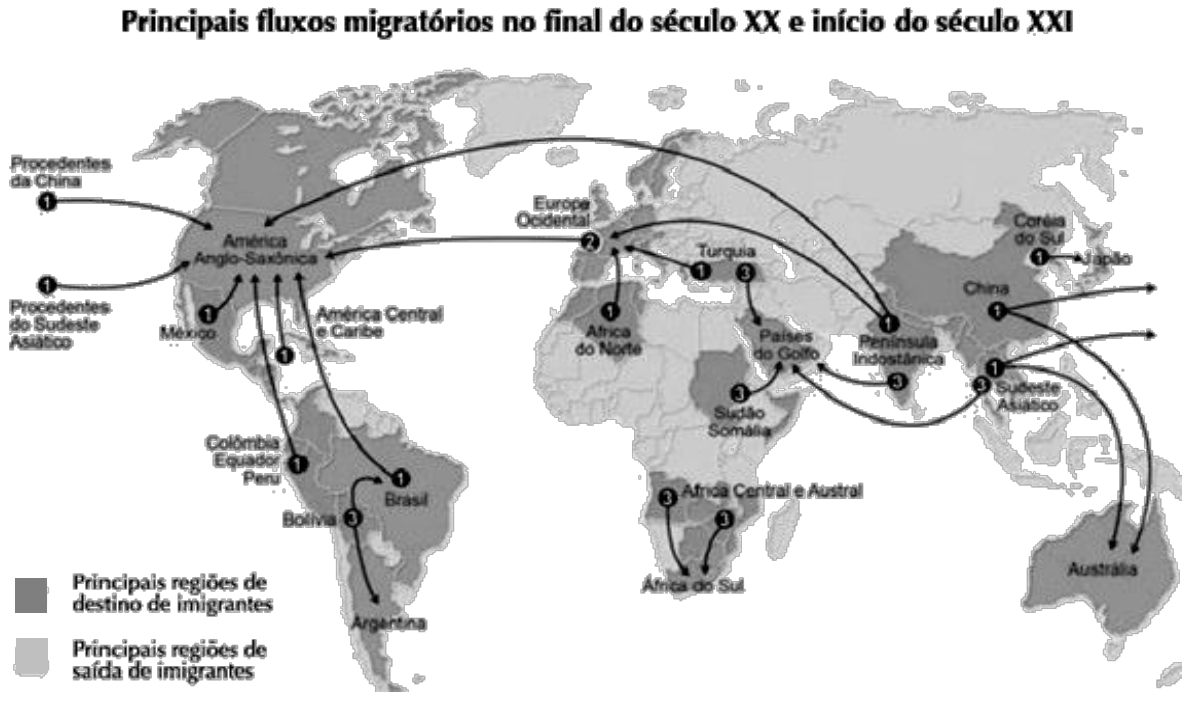
\includegraphics[width=0.95\linewidth]{static/simulados/coluni/figuras/2020/questao-34/figura-1.png}
\end{figure}
% COLUNI-AUTO-FIGURES-END

\par

Fonte: MARINUCCI, Roberto; MILESI, Rosita. \textbf{Migrações Internacionais Contemporâneas}.                 CSEM/IMDH.   Disponível   em: http://www.ufjf.br/pur/files/2011/04/MIGRA\%C3\%87\%C3\%83O-NO-MUNDO.pdf. Acesso em: 16 de ago. 2019.

\par

Com base no quadro acima, é CORRETO afirmar que:


\begin{enumerate}
\item os únicos destinos da migração internacional são os países industrializados, principalmente Estados
      Unidos, Canadá, Japão, Austrália e as nações da União Europeia.
\item muitos países desenvolvidos adotam ações excludentes para inibir o ingresso e a permanência de
      profissionais qualificados e com habilidades técnicas.
\item dentre as consequências das migrações internacionais, está o aumento da discriminação aos imigrantes,
      conhecida como homofobia.
\item um dos motivos para o aumento dos fluxos migratórios no século XXI são os movimentos vinculados às
      safras agrícolas, aos grandes projetos da construção civil e aos serviços em geral.

\end{enumerate}
